\documentclass{article}
\usepackage[utf8]{inputenc}
\usepackage{tikz}
\usetikzlibrary{positioning,shapes.geometric}
\tikzstyle{carre}=[rectangle,rounded corners,draw=red!80,fill=red!10,inner ysep=0.2cm,text width=2cm,text centered]
\tikzstyle{losange}=[diamond,draw=blue!80,fill=blue!10, inner ysep=0.1cm,text width=1cm,text centered]
\tikzstyle{cercle}=[draw,circle]
\begin{document}

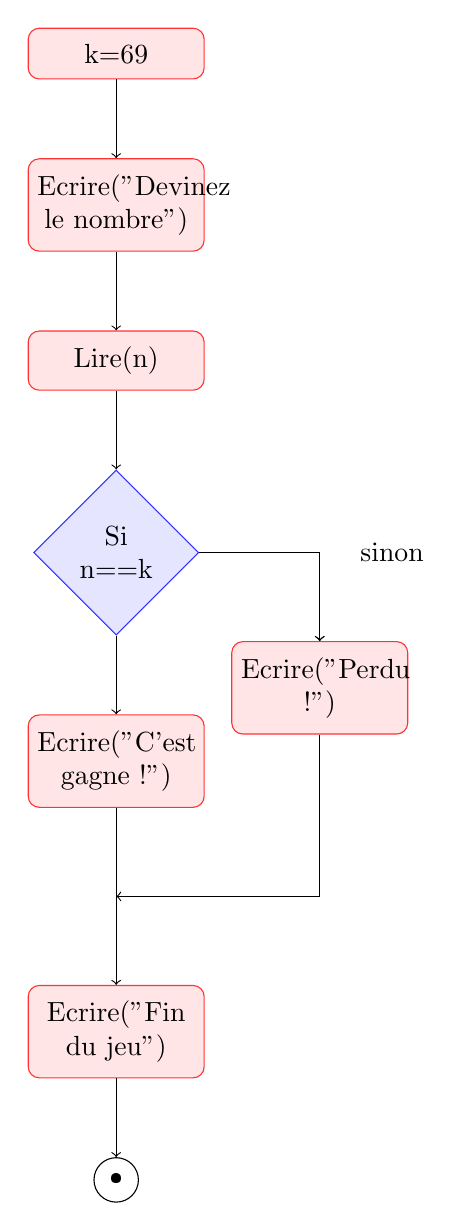
\begin{tikzpicture}

\node[carre] (A00)  {k=69};
\node[carre] (E10) [below =of A00] {Ecrire("Devinez le nombre")};
\node[carre] (L20) [below =of E10] {Lire(n)};
\node[losange] (S30) [below =of L20] {Si n$=$=k};
\node (auxS30) [right = 4em of S30]{};
\node[carre] (E40) [below =of S30] {Ecrire("C'est gagne !")};
\node (Else31) [right =4em of S30] {};
\node[carre] (E41) [below =of Else31] {Ecrire("Perdu !")};
\node (FS50) [below =of E40] {};
\node[carre] (E60) [below =of FS50] {Ecrire("Fin du jeu")};
\node[cercle] (C70) [below =of E60] {\textbullet};

\draw[->] (A00.south) to (E10.north);
\draw[->] (E10.south) to (L20.north);
\draw[->] (S30.east)|-(Else31.center)node[pos=1.3,align=center]{sinon}to(E41.north);
\draw[->] (Else31.south) to (E41.north);
\node (auxFS50) [right = 4em of FS50]{};
\draw [->](E41.south)|-(auxFS50.center)|-(FS50.center);
\draw[->] (L20.south) to (S30.north);
\draw[->] (S30.south) to (E40.north);
\draw[->] (E40.south) to (E60.north);
\draw[->] (E60.south) to (C70.north);

\end{tikzpicture}

\end{document}
